\subsection{Convertidor CC-CC Conmutado}

Para llevar a cabo el diseño del convertidor, primero debemos establecer los objetivos de rendimiento del mismo (como por ejemplo, la tensión que debe tener a la salida). Con estos valores establecidos, y junto con otras consideraciones del diseño, se van a obtener todos los parámetros que definen al convertidor, como las llaves y diodos a utilizar, tamaño de capacitores e inductores, etc.\\

\begin{figure}[h]
    \centering
    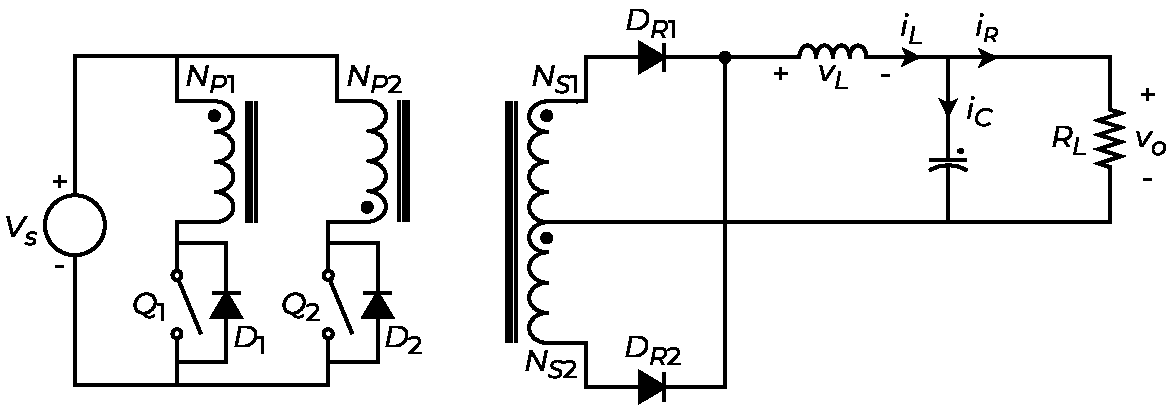
\includegraphics[scale=0.6]{Imagenes/Push-Pull.pdf}
    \caption{Diagrama del convertidor CC-CC de tipo puente completo a utilizar, con todos sus componentes (Placeholder).}
    \label{puente_completo}
\end{figure}